% font
\usepackage[default]{sourceserifpro}
\usepackage[sfdefault]{sourcesanspro}
\usepackage[scale=0.8]{sourcecodepro}

\usepackage{amsfonts} % \mathbb \mathfrak
\usepackage{mathrsfs} % \mathscr
\usepackage{makeidx}
\makeindex

% 章节标题数字样式
\ctexset{
  part/name = {,}
  part/number = \Roman{part},
  chapter/name = {,},
  chapter/number = \arabic{chapter},
  chapter/numberformat = \sf, % 数字字体 Arial
  chapter/beforeskip = 12pt, % 标题前后的间距
  chapter/afterskip = 18pt,
  chapter/fixskip = true, % 标题与正文的距离
  chapter/format += \heiti\zihao{3},  % 一级标题
  % section/name = {\S},
  section/numberformat = \rm,
  section/format += \heiti\zihao{4}\raggedright, % 二级标题
  subsection/numberformat = \rm,
  subsection/format += \heiti\zihao{-4}\raggedright,  % 三级标题
  autoindent = true,
}

% % 段首缩进
% \usepackage{indentfirst}
% \setlength{\parindent}{2em}

% https://tex.stackexchange.com/questions/354873/xelatex-sourcecodepro-listings-curly-quotes-always
\makeatletter
\defaultfontfeatures[\ttfamily]{
    Numbers   = \sourcecodepro@figurestyle ,
    Scale     = \SourceCodePro@scale ,
    Extension = .otf }

\setmonofont
		[ UprightFont    = *-\sourcecodepro@regstyle ,
		  ItalicFont     = *-\sourcecodepro@regstyle It ,
		  BoldFont       = *-\sourcecodepro@boldstyle , 
		  BoldItalicFont = *-\sourcecodepro@boldstyle It ]
		{SourceCodePro}        
\makeatother

\usepackage{titling}
\pretitle{%
  \begin{center}
  \Huge
  
\includegraphics{images/cumtb.pdf}
  \\[\bigskipamount]
  \vspace*{2cm}
}
\posttitle{
  \\[\bigskipamount]
  \vspace*{2cm}
  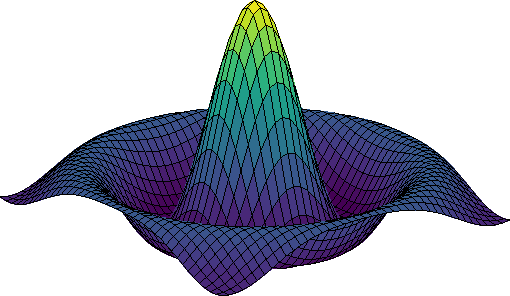
\includegraphics{images/sombrero.pdf}
  \\[\bigskipamount]
  \Large
  \end{center}
  }
% ctexbook
\RecustomVerbatimEnvironment{Highlighting}{Verbatim}{commandchars=\\\{\},formatcom=\xeCJKVerbAddon}

%%----------begin copy from https://github.com/rstudio/bookdown-----------------%%
\usepackage{framed,color}
\definecolor{shadecolor}{RGB}{248,248,248}

\renewcommand{\textfraction}{0.05}
\renewcommand{\topfraction}{0.8}
\renewcommand{\bottomfraction}{0.8}
\renewcommand{\floatpagefraction}{0.75}

\ifxetex
  \usepackage{letltxmacro}
  \setlength{\XeTeXLinkMargin}{1pt}
  \LetLtxMacro\SavedIncludeGraphics\includegraphics
  \def\includegraphics#1#{% #1 catches optional stuff (star/opt. arg.)
    \IncludeGraphicsAux{#1}%
  }%
  \newcommand*{\IncludeGraphicsAux}[2]{%
    \XeTeXLinkBox{%
      \SavedIncludeGraphics#1{#2}%
    }%
  }%
\fi

\makeatletter
\newenvironment{kframe}{%
\medskip{}
\setlength{\fboxsep}{.8em}
 \def\at@end@of@kframe{}%
 \ifinner\ifhmode%
  \def\at@end@of@kframe{\end{minipage}}%
  \begin{minipage}{\columnwidth}%
 \fi\fi%
 \def\FrameCommand##1{\hskip\@totalleftmargin \hskip-\fboxsep
 \colorbox{shadecolor}{##1}\hskip-\fboxsep
     % There is no \\@totalrightmargin, so:
     \hskip-\linewidth \hskip-\@totalleftmargin \hskip\columnwidth}%
 \MakeFramed {\advance\hsize-\width
   \@totalleftmargin\z@ \linewidth\hsize
   \@setminipage}}%
 {\par\unskip\endMakeFramed%
 \at@end@of@kframe}
\makeatother

\renewenvironment{Shaded}{\begin{kframe}}{\end{kframe}}

\newenvironment{rmdblock}[1]
  {
  \begin{itemize}
  \renewcommand{\labelitemi}{
    \raisebox{-.7\height}[0pt][0pt]{
      {\setkeys{Gin}{width=3em,keepaspectratio}\includegraphics{images/#1}}
    }
  }
  \setlength{\fboxsep}{1em}
  \begin{kframe}
  \item
  }
  {
  \end{kframe}
  \end{itemize}
  }
\newenvironment{rmdnote}
  {\begin{rmdblock}{note}}
  {\end{rmdblock}}
\newenvironment{rmdcaution}
  {\begin{rmdblock}{caution}}
  {\end{rmdblock}}
\newenvironment{rmdimportant}
  {\begin{rmdblock}{important}}
  {\end{rmdblock}}
\newenvironment{rmdtip}
  {\begin{rmdblock}{tip}}
  {\end{rmdblock}}
\newenvironment{rmdwarning}
  {\begin{rmdblock}{warning}}
  {\end{rmdblock}}

%%----------end copy from https://github.com/rstudio/bookdown-----------------%%
% for kableExtra
% \usepackage[table]{xcolor}

\usepackage{tikz,everypage}

\makeatletter
\global\let\tikz@ensure@dollar@catcode=\relax
\makeatother

%%--------- 每页第一列为行号 -----------%%
\makeatletter
\AtBeginDocument{%
  \AddEverypageHook{%
    \small
    \begin{tikzpicture}[remember picture,overlay]
      \path (current page.north west) --  (current page.south west)
            \foreach \i in {1,...,\fakelinenos}
               { node [pos={(\i-.5)/\fakelinenos},
                  xshift=\fakelinenoshift, line number style] {\i} }  ;
    \end{tikzpicture}%
  }%
}
\makeatother
\tikzset{%
  line numbers/.store in=\fakelinenos,
  line numbers=72,
  line number shift/.store in=\fakelinenoshift,
  line number shift=5mm,
  line number style/.style={text=gray},
}

%% 添加水印 Draft
\usepackage{draftwatermark}
\SetWatermarkText{DRAFT}
\SetWatermarkLightness{0.9}
\usepackage{background}
\SetBgContents{仅供学习使用,不得用于商业目的。
\url{https://github.com/XiangyunHuang/notesdown}}
\SetBgScale{1}
\SetBgAngle{0}
\SetBgOpacity{1}
\SetBgColor{red}
\SetBgPosition{current page.north}
\SetBgVshift{-0.5cm}

\frontmatter
